\documentclass[11pt,letterpaper]{article}

% ---------------------------------------------------------------
%  Motor-cage output joint: bolt slip and gusset bracket validation
%  Compile:  latexmk -pdf main.tex   (pdfLaTeX, TeX Live 2023+)
% ---------------------------------------------------------------
\usepackage[T1]{fontenc}
\usepackage[sc]{mathpazo}
\linespread{1.05}
\usepackage[margin=1in]{geometry}
\usepackage{microtype}
\usepackage{amsmath,amssymb}
\usepackage{graphicx}
\usepackage{booktabs}
\usepackage{threeparttable}
\usepackage{siunitx}
\usepackage{caption}
\usepackage{subcaption}
\usepackage{float}
\usepackage{enumitem}
\usepackage{xcolor}
\usepackage{tikz}
\usepackage{pgfplots}
\pgfplotsset{compat=1.18}
\usepackage[hidelinks]{hyperref}
\usepackage[capitalise,noabbrev]{cleveref}

\graphicspath{{figures/}}
\sisetup{group-minimum-digits=4, range-phrase=--, detect-weight=true}
\captionsetup{font=small,labelfont=bf}
\setlist{itemsep=2pt,topsep=4pt}

% chart colours (categorical slots 1-3, validated palette) and diagram ink
\definecolor{s1}{HTML}{2A78D6}
\definecolor{s2}{HTML}{EB6834}
\definecolor{s3}{HTML}{1BAF7A}
\definecolor{ink}{HTML}{2B2F33}
\definecolor{muted}{HTML}{8A9196}

\newcommand{\Nm}{\si{\newton\metre}}

\title{\textbf{Torsional Analysis of an Exoskeleton Motor-Cage Output Joint}\\[4pt]
\large Bolt-Slip Prediction and Gusset-Bracket Validation with Preloaded-Bolt FEA}
\author{Tien-Hao Chen\\University of California, San Diego}
\date{November 2026}

\begin{document}
\maketitle

\begin{abstract}
\noindent
The output side of an upper-limb exoskeleton joint transmits the torque of a CubeMars
AKH70-16 actuator (rated \SI{26}{\newton\metre}, peak \SI{78}{\newton\metre}) from the
rotor flange to the next link through a 4$\times$M4 bolted joint between two
\SI{12.7}{mm} (\SI{0.5}{in}) 6061-T6 plates. A bolt-group hand calculation showed that, at
peak torque, the required shear on the outermost bolt (\SI{1494}{\newton}) exceeds the
friction capacity of a preloaded M4 joint (\SI{593}{\newton}), so the joint would slip.
Two L-shaped gusset brackets were added. A SolidWorks Simulation static study with
12 preloaded bolt connectors, frictional contact and a three-level mesh-convergence
check shows that the brackets reduce the shear on the original bolts by a factor of
\num{32}, keep every joint below the slip threshold, and increase the torsional
stiffness of the output joint by a factor of \num{8.9}. The highest converged stress in
the bracket is \SI{55}{MPa} (static safety factor \num{5.0}); the highest converged
stress in the assembly, \SI{208}{MPa}, is preload bearing at a bolt-hole edge and
motivates the use of washers.
\end{abstract}

% =================================================================
\section{Objective and scope}
% =================================================================
The motor cage holds the AKH70-16 stator on the input side and carries its rotor output
to the next link on the output side. The output load path studied here is
\begin{center}
rotor flange $\rightarrow$ Rotating Spacer ($\varnothing$50$\times$15)
$\rightarrow$ Moving Side Plate (\SI{12.7}{mm})
$\rightarrow$ 4$\times$M4 $\rightarrow$ Static Connector (\SI{12.7}{mm})
$\rightarrow$ shaft support,
\end{center}
with two 5\,mm Bracket gussets bolted across the corner between the Moving Side Plate
and the Static Connector as a parallel path. The analysis answers two questions:
\begin{enumerate}
  \item Without the brackets, does the 4$\times$M4 joint slip at peak torque?
  \item With the brackets, how far is the bolt shear reduced, how much stiffer is the
        joint, and how highly stressed are the brackets themselves?
\end{enumerate}
The input (stator) side, the actuator internals and the shaft supports are outside the
scope of this report.

% =================================================================
\section{Hand calculations}
% =================================================================
\subsection{Bolt preload and friction capacity}
For an M4 class 8.8 screw (tensile stress area $A_s=\SI{8.78}{mm^2}$, proof strength
$S_p=\SI{600}{MPa}$) tightened to \SI{75}{\percent} of proof,
\begin{equation}
  F_i = 0.75\,S_p A_s = 0.75(600)(8.78) \approx \SI{3950}{\newton},
\end{equation}
which with a nut factor $K=0.2$ corresponds to a tightening torque
\begin{equation}
  T_{\text{tighten}} = K F_i d = 0.2(3950)(0.004) \approx \SI{3.2}{\newton\metre}.
\end{equation}
With a single faying surface and $\mu=0.15$, the shear a bolt can transmit by friction
before slipping is
\begin{equation}
  F_{\text{slip}} = \mu F_i = 0.15(3950) \approx \SI{593}{\newton}.
\end{equation}

\subsection{Bolt-group shear}
The 4$\times$M4 joint is a bolt group loaded by a pure in-plane moment equal to the motor
torque $T$. Assuming the plates are rigid and all of $T$ is carried by bolt shear, the
force on bolt $i$ at distance $r_i$ from the group centroid is
\begin{equation}
  F_i = \frac{T\,r_i}{\sum_j r_j^2}.
  \label{eq:boltgroup}
\end{equation}
The four bolts lie on one line at $x=\pm\SI{9}{mm}$ and $\pm\SI{22.5}{mm}$, so
$\sum r^2 = 2(9^2+22.5^2)=\SI{1174.5}{mm^2}$. Adding the four bracket screws on the plate
edges (at \SI{38.1}{mm} and \SI{57.0}{mm} from the centroid) and treating the brackets as
rigid raises $\sum r^2$ to about \SI{10576}{mm^2}. \Cref{fig:boltgroup} shows the
geometry and \cref{tab:hand} the results.

\begin{figure}[H]
\centering
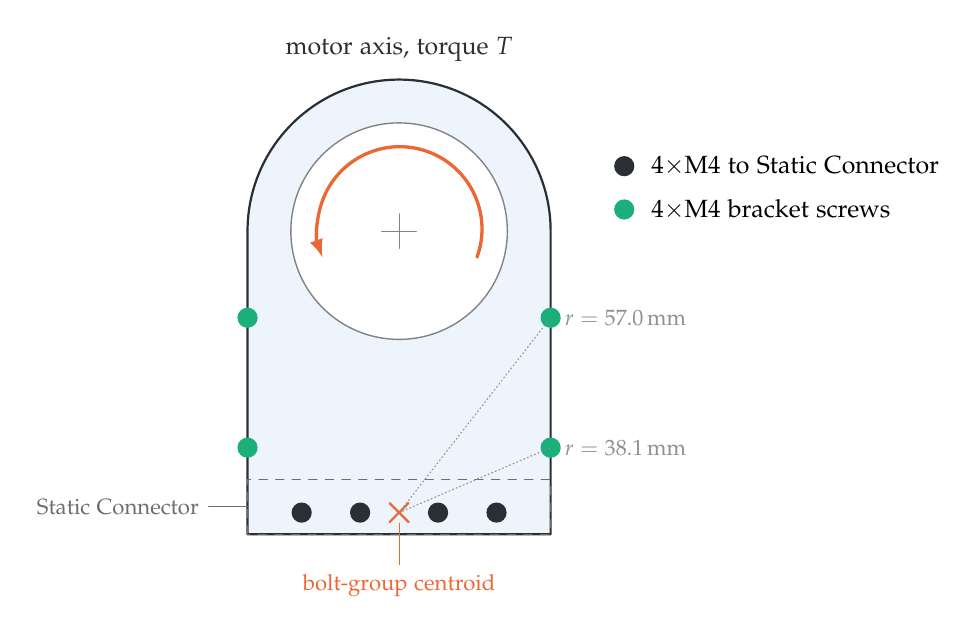
\begin{tikzpicture}[scale=0.055, line cap=round, line join=round, font=\small]
  % Moving Side Plate outline (local coords, mm): rectangle + R35 half-disc
  \draw[ink, line width=0.8pt, fill=s1!8]
     (35,-70) -- (35,0) arc (0:180:35) -- (-35,-70) -- cycle;
  % Rotating spacer and motor axis
  \draw[ink!60, line width=0.5pt, fill=white] (0,0) circle (25);
  \draw[ink!60] (-4,0) -- (4,0) (0,-4) -- (0,4);
  \node[ink, anchor=south] at (0,37) {motor axis, torque $T$};
  \draw[-{latex}, s2, line width=1.2pt] (18,-6) arc (-20:200:19);
  % Static Connector footprint (end face on the plate)
  \draw[ink!70, dashed] (-35,-70) rectangle (35,-57.3);
  \draw[ink!70] (-35,-63.6) -- (-44,-63.6) node[anchor=east, font=\footnotesize] {Static Connector};
  % original 4xM4
  \foreach \x in {-22.5,-9,9,22.5}
     \filldraw[ink] (\x,-65) circle (2.2);
  % centroid
  \draw[s2, line width=0.8pt] (-2.2,-62.8) -- (2.2,-67.2) (-2.2,-67.2) -- (2.2,-62.8);
  \draw[s2] (0,-67.5) -- (0,-77) node[anchor=north, font=\footnotesize] {bolt-group centroid};
  % bracket screws on the edges
  \foreach \y in {-50,-20} {
     \filldraw[s3] (35,\y) circle (2.2);
     \filldraw[s3] (-35,\y) circle (2.2);
  }
  % dimension r to bracket screw
  \draw[muted, densely dotted] (0,-65) -- (35,-20);
  \node[muted, anchor=west] at (36,-20) {\footnotesize $r=\SI{57.0}{mm}$};
  \draw[muted, densely dotted] (0,-65) -- (35,-50);
  \node[muted, anchor=west] at (36,-50) {\footnotesize $r=\SI{38.1}{mm}$};
  % legend
  \filldraw[ink] (52,15) circle (2.2); \node[anchor=west] at (56,15) {4$\times$M4 to Static Connector};
  \filldraw[s3] (52,5) circle (2.2);  \node[anchor=west] at (56,5) {4$\times$M4 bracket screws};
\end{tikzpicture}
\caption{Moving Side Plate (top view, plate coordinates). The 4$\times$M4 joint is a single
row spanning only \SI{45}{mm}; the bracket screws add load points far from the centroid.}
\label{fig:boltgroup}
\end{figure}

\begin{table}[H]
\centering
\caption{Hand-calculation results.}
\label{tab:hand}
\begin{tabular}{@{}lS[table-format=4.0]S[table-format=3.0]@{}}
\toprule
Quantity & {Peak, \SI{78}{\newton\metre}} & {Rated, \SI{26}{\newton\metre}}\\
\midrule
Rotor 6$\times$M4 on PCD\,35, shear per bolt                 & 743  & 248 \\
4$\times$M4, outer bolt shear, no bracket                     & 1494 & 498 \\
4$\times$M4, outer bolt shear, rigid bracket                  & 166  & 55  \\
Bracket screw, maximum shear, rigid bracket                   & 420  & 140 \\
\midrule
Friction capacity per M4, $F_{\text{slip}}$                   & \multicolumn{2}{c}{593} \\
\bottomrule
\end{tabular}
\\[4pt]
{\footnotesize All forces in newtons.}
\end{table}

Without the brackets the outer bolt needs \SI{1494}{\newton} against a capacity of
\SI{593}{\newton}; the joint is predicted to slip at peak torque and to be marginal
(\SI{498}{\newton}) even at rated torque. With rigid brackets every bolt stays well below
the slip threshold.

\subsection{Bearing under the screw head}
The preload acts on the annulus between the \SI{7}{mm} head and the \SI{4.3}{mm} hole:
\begin{equation}
  p = \frac{F_i}{\tfrac{\pi}{4}(7^2-4.3^2)} = \frac{3950}{\SI{24.0}{mm^2}}
    \approx \SI{165}{MPa},
\end{equation}
below the bearing yield strength of 6061-T6 (about \SI{386}{MPa}) but high enough that
embedding and preload loss are a concern for an aluminium joint under cyclic load.

% =================================================================
\section{Finite-element model}
% =================================================================
\Cref{tab:setup} summarises the study, which was built in SOLIDWORKS Simulation
(Premium for Students 2026 SP4.1) on a dedicated configuration in which the actuator,
the input-side plates, the Moving Connector, the shaft supports and the spacers are
suppressed. \Cref{fig:setup} shows the boundary conditions and mesh.

\begin{table}[H]
\centering
\caption{Simulation set-up.}
\label{tab:setup}
\begin{tabular}{@{}p{0.27\linewidth}p{0.66\linewidth}@{}}
\toprule
Item & Setting \\
\midrule
Study type & Linear static, FFEPlus solver, small displacement \\
Bodies & Rotating Spacer, Moving Side Plate, Static Connector, Bracket\,1, Bracket\,2 \\
Material & 6061-T6: $E=\SI{69}{GPa}$, $\nu=0.33$, $S_y=\SI{275}{MPa}$ \\
Global interaction & Contact (no penetration), $\mu=0.15$ \\
Local interaction & Rotating Spacer $\leftrightarrow$ Moving Side Plate bonded
   (clamped by the rotor screws; not the joint under study) \\
Bolt connectors & 12 $\times$ ``standard or counterbore screw'': 4 plate-to-connector,
   8 bracket screws. Head \SI{7}{mm}, shank \SI{4}{mm}, alloy steel, distributed
   coupling, axial preload \SI{3950}{\newton} \\
Fixture & Fixed geometry on the four M6 tapped-hole faces of the Static Connector
   (attachment to the shaft support) \\
Load & Remote load, rigid connection, on the rotor-side face of the Rotating Spacer;
   moment \SI{78}{\newton\metre} about the motor axis \\
Mesh & Curvature-based, second-order tetrahedra; see \cref{tab:conv} \\
\bottomrule
\end{tabular}
\end{table}

\begin{figure}[H]
\centering
\begin{subfigure}[t]{0.32\linewidth}\centering
  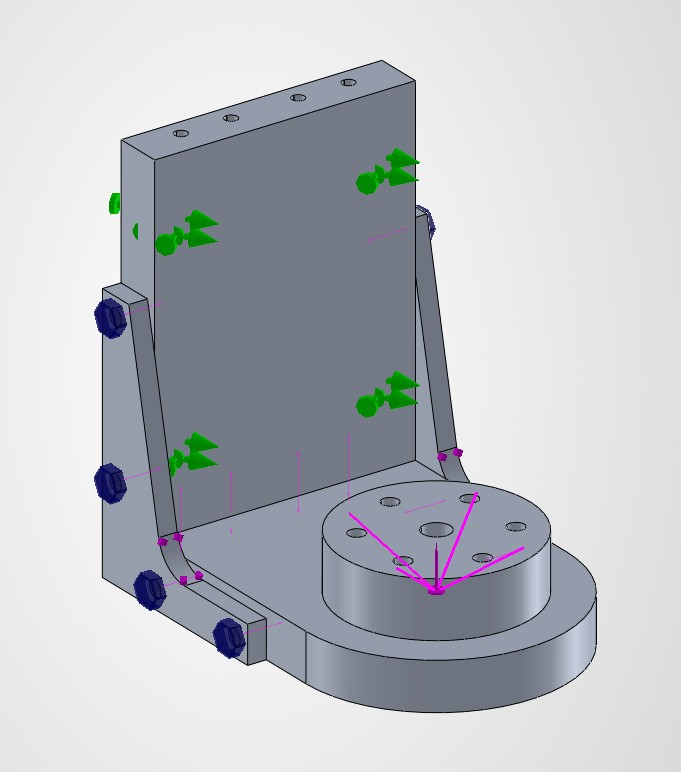
\includegraphics[width=\linewidth]{setup_bc.jpg}
  \caption{Fixtures (green), torque (magenta) and bolt connectors.}
\end{subfigure}\hfill
\begin{subfigure}[t]{0.32\linewidth}\centering
  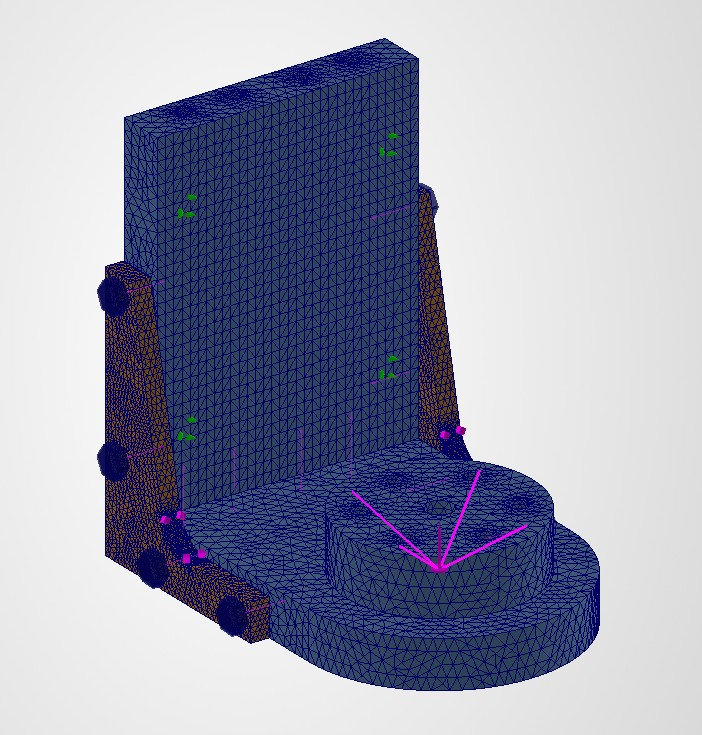
\includegraphics[width=\linewidth]{mesh_overview.jpg}
  \caption{Mesh, fine2 level.}
\end{subfigure}\hfill
\begin{subfigure}[t]{0.32\linewidth}\centering
  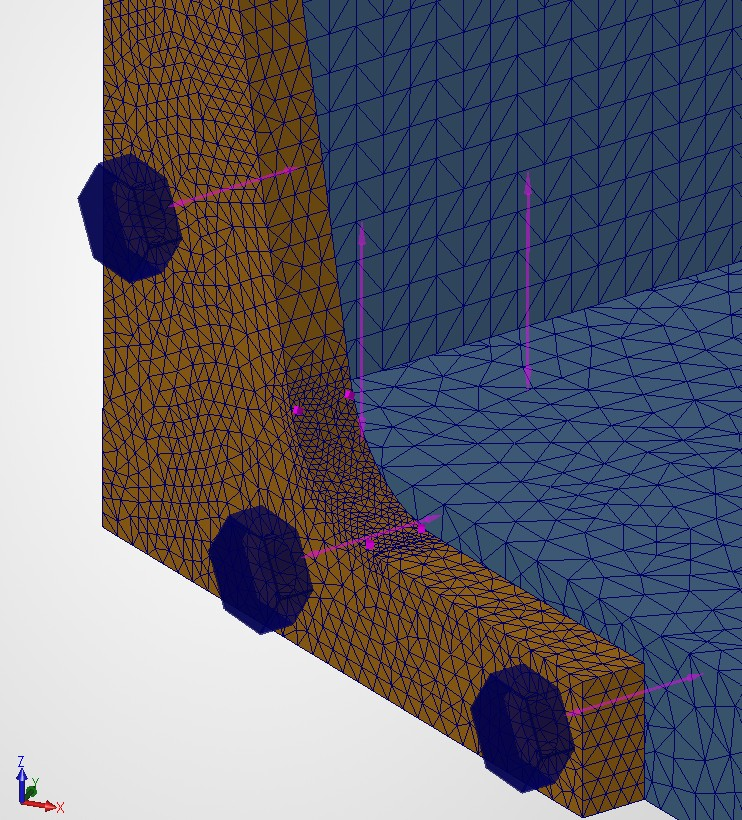
\includegraphics[width=\linewidth]{mesh_fillet.jpg}
  \caption{Local refinement at the bracket R10 fillet.}
\end{subfigure}
\caption{Model, boundary conditions and mesh.}
\label{fig:setup}
\end{figure}

% =================================================================
\section{Mesh convergence}
% =================================================================
Three meshes were run with brackets fitted. \emph{fine} refines the two side faces of the
Moving Side Plate that the brackets bear on; \emph{fine2} additionally refines the brackets.
\Cref{tab:conv} lists the quantities used in the conclusions.

\begin{table}[H]
\centering
\begin{threeparttable}
\caption{Convergence of the with-bracket study (peak torque).}
\label{tab:conv}
\small\setlength{\tabcolsep}{5pt}
\begin{tabular}{@{}llllr@{}}
\toprule
 & coarse & fine & fine2 & $\Delta$ fine$\to$fine2\\
\midrule
Elements                            & 250\,765 & 529\,313 & 846\,763 & \\
Global max / min size (mm)          & 3 / 0.5 & 3 / 0.5 & 3 / 0.3 & \\
Mesh controls (mm)\tnote{a}         & 0.6 / 1.5 / -- & 0.6 / 1.5 / 0.4 & 0.3 / 0.75 / 0.4 & \\
\midrule
Max displacement (mm)               & 0.09318 & 0.09303 & 0.09296 & $-0.1\%$ \\
R10 fillet, mean (MPa)              & 22.78 & 23.43 & 23.10 & $-1.4\%$ \\
R10 fillet, max (MPa)               & 55.33 & 55.43 & 55.37 & $-0.1\%$ \\
Bolt-hole edge, mean (MPa)\tnote{b} & 138.0 & 178.7 & 177.3 & $-0.8\%$ \\
Bolt-hole edge, max (MPa)\tnote{b}  & 219.8 & 206.2 & 208.0 & $+0.9\%$ \\
Max bolt shear (N)\tnote{c}         & 119.8 & -- & 119.4 & $-0.3\%$ \\
Global max von Mises (MPa)          & 219.8 & 230.5 & 237.6 & $+3.1\%$, singular \\
\bottomrule
\end{tabular}
\begin{tablenotes}\footnotesize
\item[a] R10 fillet faces / bracket bodies / plate side faces.
\item[b] Bracket\,2, hole $(50,5)$, edge on the face clamped against the Moving Side Plate.
\item[c] Bolt forces were exported for coarse and fine2 only; $\Delta$ is coarse$\to$fine2.
\end{tablenotes}
\end{threeparttable}
\end{table}

Displacement, bolt shear and the bracket-fillet stress converge within \SI{1.5}{\percent}.
The bolt-hole edge changes by \SI{30}{\percent} from coarse to fine because its
\emph{contact partner}, the side face of the plate, is refined; once both sides of the
interface are fine it changes by less than \SI{1}{\percent} (\cref{fig:edge}). The global
maximum keeps rising and moves location between meshes; it sits on bolt-connector and
contact-edge singularities and is not used for design.

\begin{figure}[H]
\centering
\begin{tikzpicture}
\begin{axis}[
  width=0.82\linewidth, height=6.2cm,
  xlabel={Normalised position along hole edge},
  ylabel={von Mises stress (MPa)},
  xmin=0, xmax=1, ymin=100, ymax=230,
  axis lines=left, axis line style={muted},
  tick style={muted}, tick label style={font=\small, text=ink},
  label style={font=\small, text=ink},
  ymajorgrids, grid style={muted!25, line width=0.3pt},
  legend style={draw=none, font=\small, at={(0.5,1.02)}, anchor=south, legend columns=3},
  legend cell align=left,
  every axis plot/.append style={line width=1.2pt},
]
\addplot[s1, mark=*, mark size=1.4pt] table[x=s,y=vm]{data/edge_coarse.dat};
\addlegendentry{coarse (251k)}
\addplot[s2, mark=square*, mark size=1.3pt, densely dashed] table[x=s,y=vm]{data/edge_fine.dat};
\addlegendentry{fine (529k)}
\addplot[s3, mark=triangle*, mark size=1.7pt] table[x=s,y=vm]{data/edge_fine2.dat};
\addlegendentry{fine2 (847k)}
\addplot[muted, line width=0.6pt, dashed, domain=0:1, samples=2] {165};
\node[anchor=north west, font=\scriptsize, text=ink!70, fill=white, inner sep=1pt] at (axis cs:0.6,163) {hand calc.\ head bearing, 165 MPa};
\end{axis}
\end{tikzpicture}
\caption{von Mises stress around the clamped edge of bracket hole $(50,5)$ for the three
meshes. The coarse curve has single-node spikes; fine and fine2 overlap.}
\label{fig:edge}
\end{figure}

% =================================================================
\section{Results with the brackets}
% =================================================================
\subsection{Bolt forces}
All 12 connectors hold their preload (\SIrange{3917}{3976}{\newton}). The largest shear on
any bolt is \SI{119}{\newton}, a fifth of the friction capacity, so no joint slips at peak
torque. The four plate-to-connector bolts carry \SIrange{6}{25}{\newton}
(\cref{tab:bolts}); their bending moments are below \SI{0.25}{\newton\metre}.

The FEA shear is far below the rigid-bracket hand estimate because the hand calculation
routes all torque through bolt shear. In the model, preload clamps the faying surfaces and
most of the torque is carried by friction and contact pressure; bolt shanks see only
the small elastic mismatch. This is the intended behaviour of a preloaded joint.

\subsection{Stress and displacement}
\begin{figure}[H]
\centering
\begin{subfigure}[t]{0.32\linewidth}\centering
  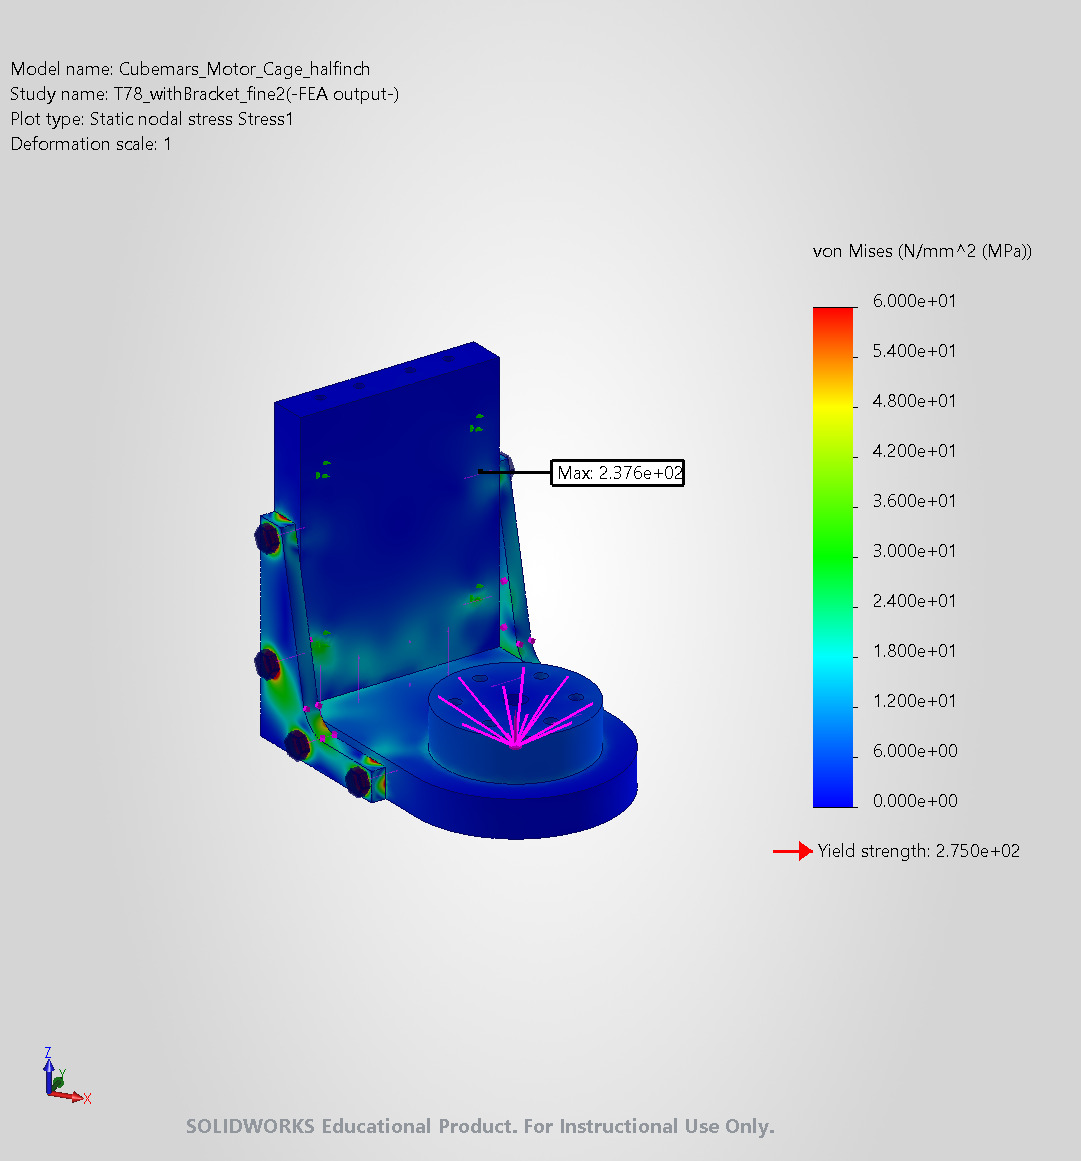
\includegraphics[width=\linewidth]{withBracket_fine2_stress_iso.jpg}
  \caption{von Mises, \SIrange{0}{60}{MPa} scale.}
\end{subfigure}\hfill
\begin{subfigure}[t]{0.32\linewidth}\centering
  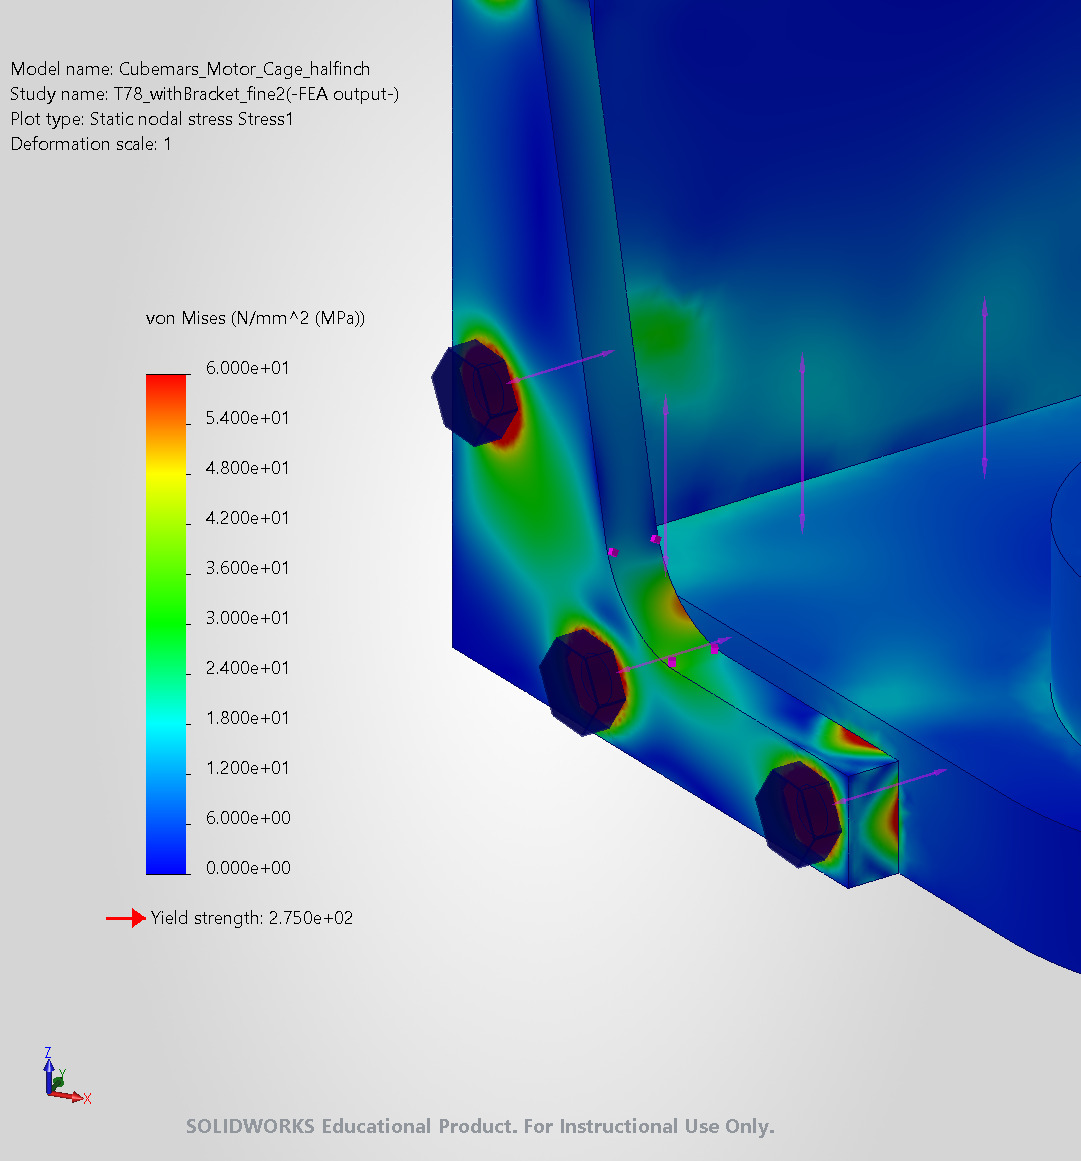
\includegraphics[width=\linewidth]{withBracket_fine2_stress_fillet.jpg}
  \caption{Bracket corner and R10 fillet.}
\end{subfigure}\hfill
\begin{subfigure}[t]{0.32\linewidth}\centering
  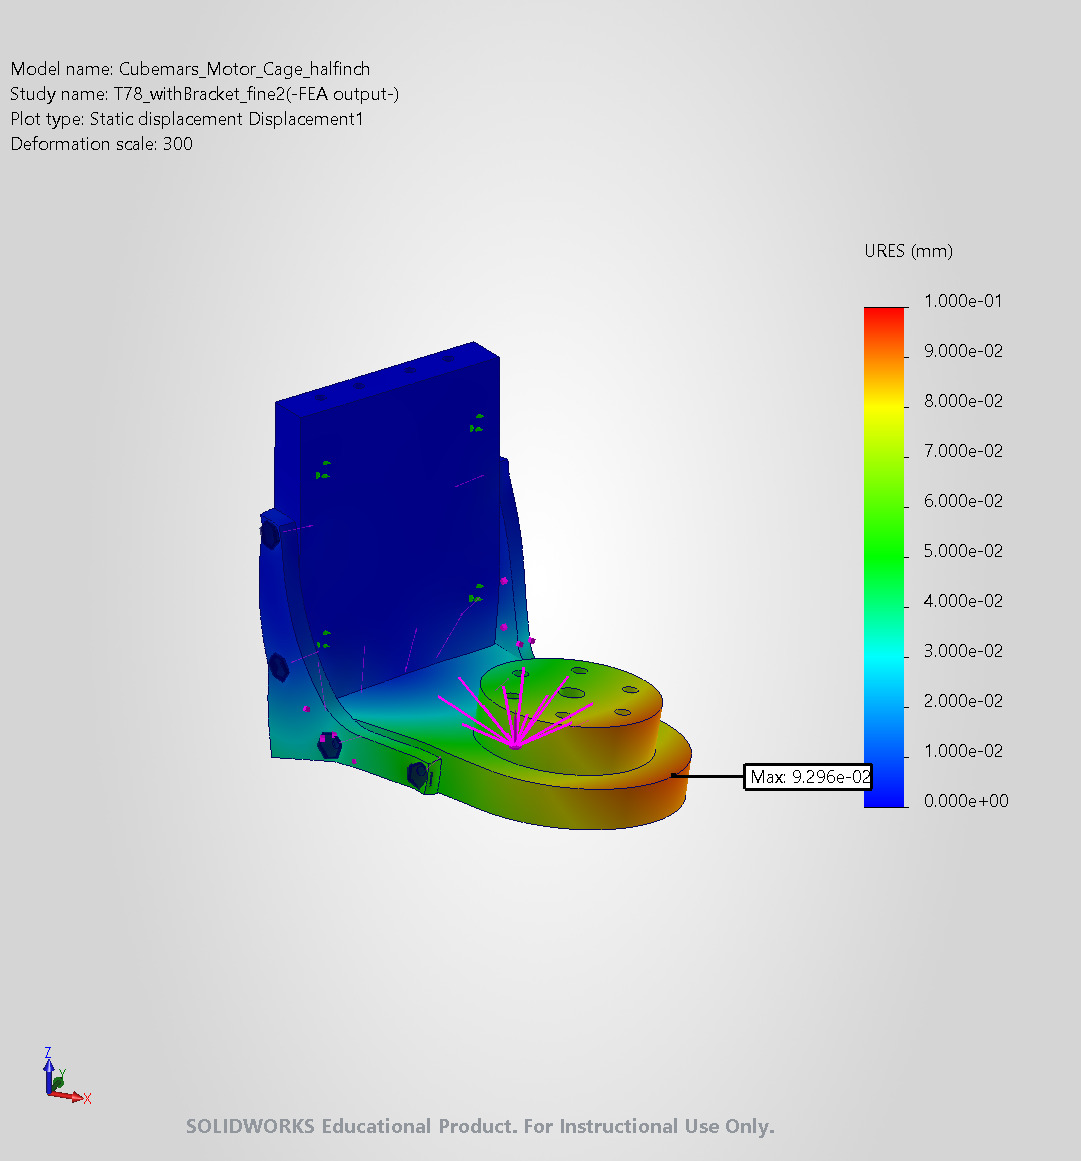
\includegraphics[width=\linewidth]{withBracket_fine2_disp_iso.jpg}
  \caption{Resultant displacement, $300\times$.}
\end{subfigure}
\caption{With brackets, fine2 mesh, peak torque.}
\label{fig:with}
\end{figure}

\begin{itemize}
  \item \textbf{Bracket fillet.} Mean \SI{23}{MPa}; maximum \SI{55}{MPa} at the inner face
        where the plate corner, the Static Connector end face and the bracket meet. The
        maximum is mesh-independent (\cref{tab:conv}), so it is treated as a real local
        concentration: static safety factor $275/55=5.0$, and $96/55\approx1.7$ against the
        fatigue strength of 6061-T6 at $5\times10^8$ cycles for fully reversed loading.
  \item \textbf{Bolt-hole edges.} \SIrange{150}{208}{MPa} around the clamped face of the
        bracket holes, consistent with the \SI{165}{MPa} head-bearing estimate. This
        stress is set by preload, is compressive and barely changes with joint torque,
        so it is a static rather than a fatigue concern; local safety factor
        $275/208\approx1.3$.
  \item \textbf{Displacement.} Maximum \SI{0.093}{mm} at the far edge of the plate.
\end{itemize}

% =================================================================
\section{Comparison: without the brackets}
% =================================================================
A copy of the coarse study with both brackets excluded and their eight connectors deleted
isolates the effect of the brackets. Coarse-level results are adequate for this comparison
because displacement and bolt shear converge within \SI{0.4}{\percent} (\cref{tab:conv}).

\subsection{Rotation angle}
Without the brackets the plate rotates about the bolt row, not about the motor axis
(\cref{fig:without}). The displacement ratio around the rim of the
\SI{50}{mm} spacer confirms a near-rigid rotation:
$u_{\min}/u_{\max}=0.375/0.849=0.44$, equal to the ratio of the rim's nearest and farthest
distances from the bolt row, $40/90=0.44$. Because the pivot is not on the motor axis, the
rotation angle is taken from the displacement difference across the rim diameter $D$,
which is independent of the pivot location:
\begin{equation}
  \theta \approx \frac{u_{\max}-u_{\min}}{D}, \qquad K_\theta = \frac{T}{\theta}.
\end{equation}

\begin{table}[H]
\centering
\caption{With versus without brackets, peak torque, coarse mesh.}
\label{tab:bolts}
\begin{tabular}{@{}lS[table-format=5.3]S[table-format=5.3]r@{}}
\toprule
 & {With brackets} & {Without} & Ratio \\
\midrule
Screw\,1, outer, shear (N)        & 24.8  & 768.6 & $\times31$ \\
Screw\,2, inner, shear (N)        & 7.6   & 283.6 & $\times37$ \\
Screw\,3, inner, shear (N)        & 6.0   & 295.8 & $\times49$ \\
Screw\,4, outer, shear (N)        & 20.6  & 782.7 & $\times38$ \\
Max bolt bending moment (\si{\newton\metre}) & 0.23 & 6.72 & $\times29$ \\
Joint state                       & {no slip} & {slip} & \\
\midrule
Max displacement (mm)             & 0.093 & 0.935 & $\times10$ \\
Spacer rim $u_{\max}$ / $u_{\min}$ (mm) & {0.0920 / 0.0387} & {0.849 / 0.375} & \\
Rotation $\theta$ (deg)           & 0.061 & 0.543 & $\times8.9$ \\
Torsional stiffness $K_\theta$ (\si{\kilo\newton\metre\per\radian}) & 73.2 & 8.2 & $\times8.9$ \\
Tip motion of a \SI{300}{mm} link (mm) & 0.32 & 2.8 & \\
\bottomrule
\end{tabular}
\end{table}

\begin{figure}[H]
\centering
\begin{subfigure}[t]{0.32\linewidth}\centering
  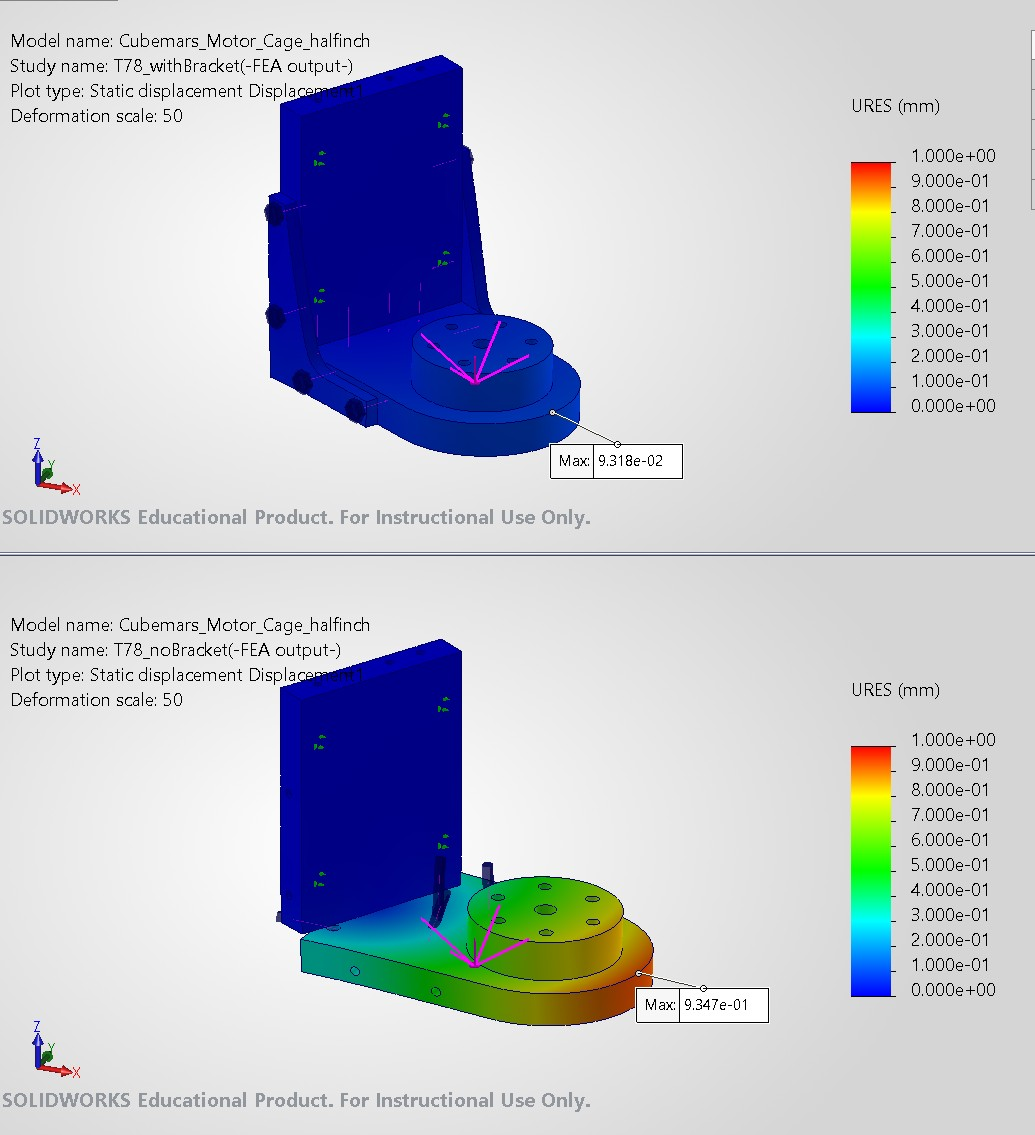
\includegraphics[width=\linewidth]{compare_disp.jpg}
  \caption{Displacement, common \SIrange{0}{1}{mm} scale, $50\times$; with (top) and
           without (bottom) brackets.}
\end{subfigure}\hfill
\begin{subfigure}[t]{0.32\linewidth}\centering
  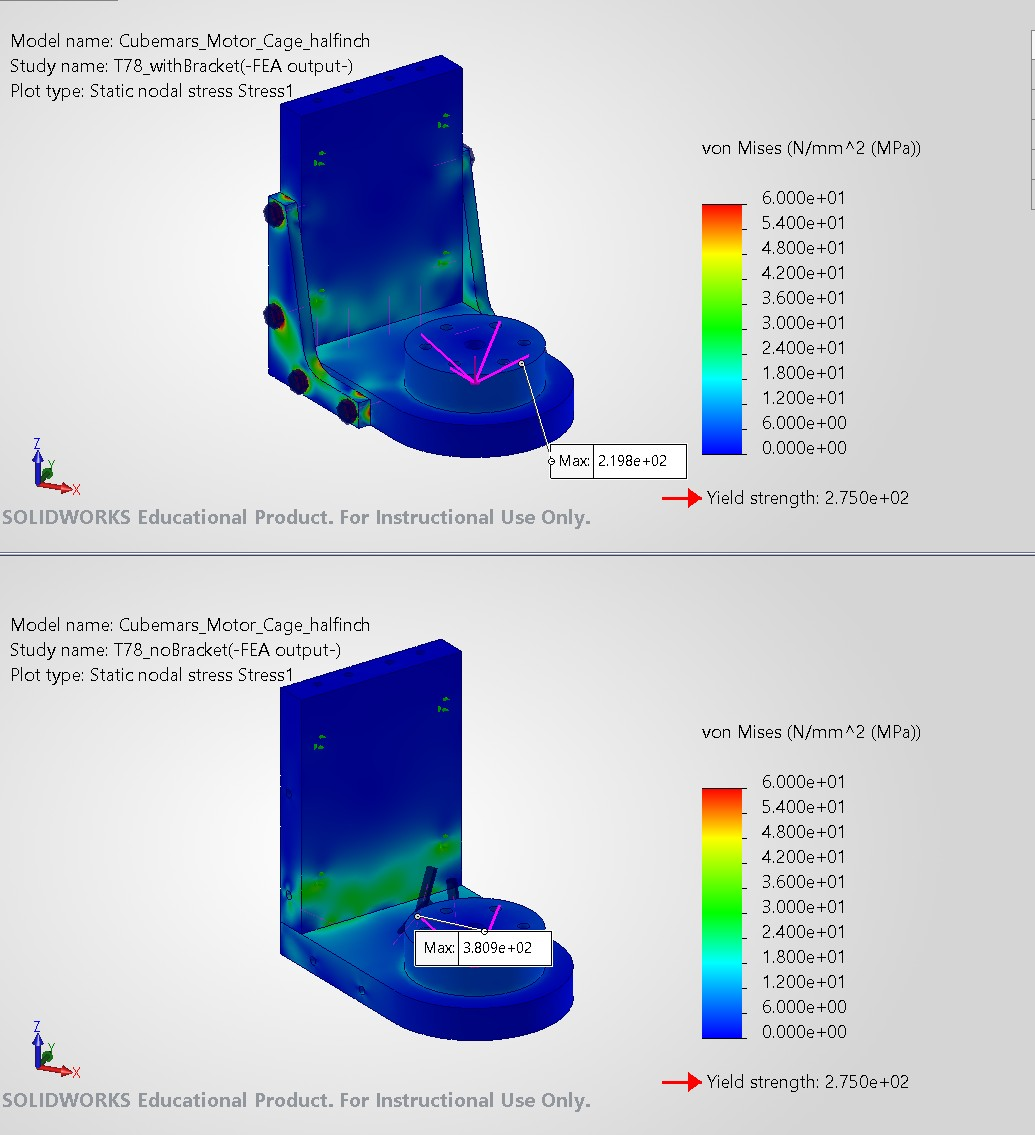
\includegraphics[width=\linewidth]{compare_stress.jpg}
  \caption{von Mises, common \SIrange{0}{60}{MPa} scale; with (top) and without (bottom).}
\end{subfigure}\hfill
\begin{subfigure}[t]{0.32\linewidth}\centering
  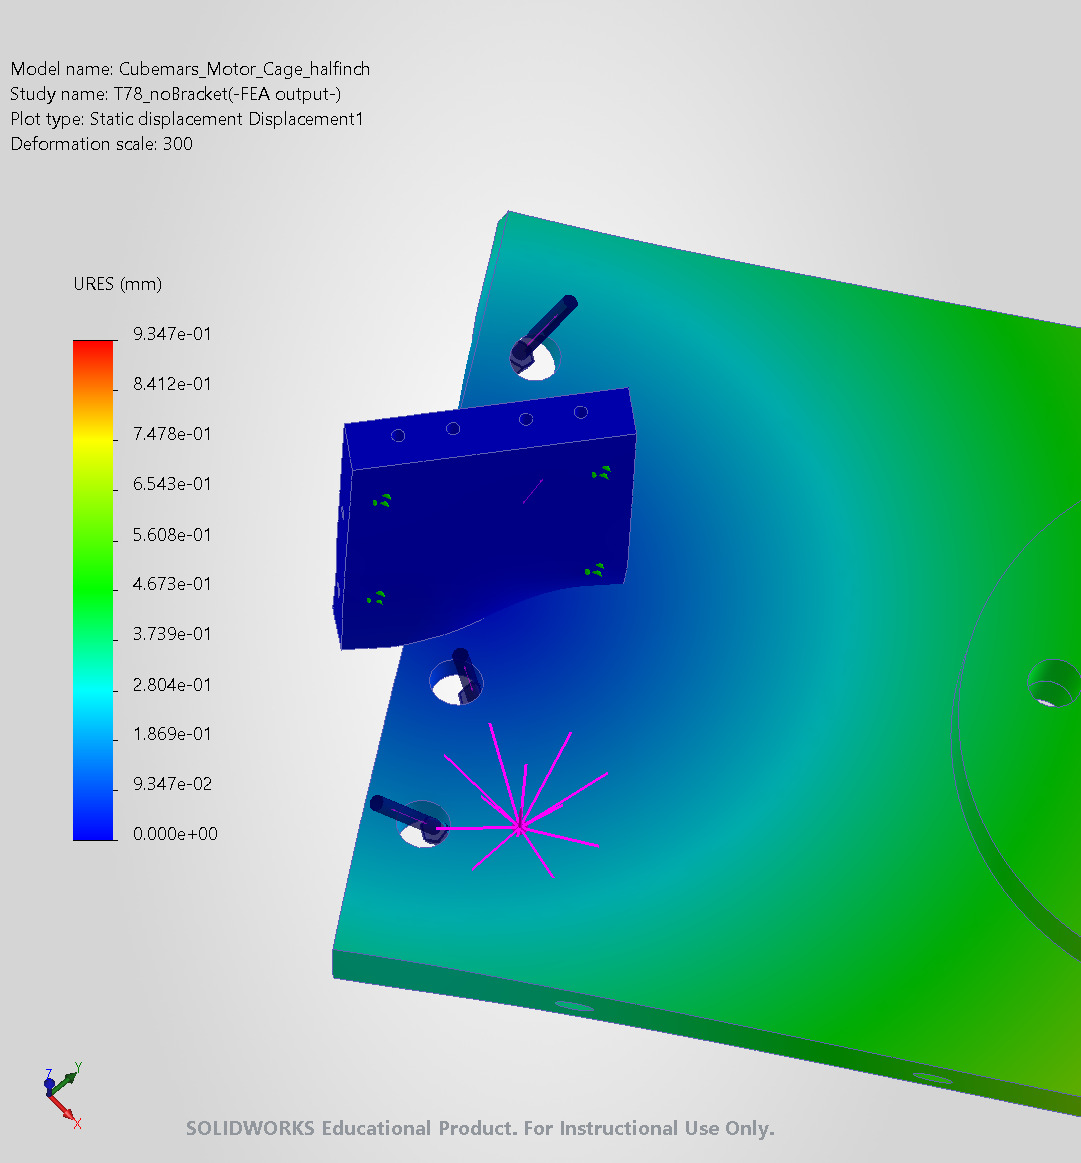
\includegraphics[width=\linewidth]{noBracket_coarse_disp_zoom_in.jpg}
  \caption{Without brackets, $300\times$: the plate swings about the bolt row.}
\end{subfigure}
\caption{Effect of removing the brackets.}
\label{fig:without}
\end{figure}

\subsection{Interpretation}
\begin{itemize}
  \item The outer bolts carry \SIrange{770}{783}{\newton}, above the
        \SI{593}{\newton} friction capacity: the joint slips, as the hand calculation
        predicted.
  \item The outer-to-inner shear ratio, $775/290=2.7$, is close to the bolt-group ratio
        $22.5/9=2.5$ from \cref{eq:boltgroup}, which supports the model.
  \item The bolt shear accounts for
        $2(775.7)(22.5)+2(289.7)(9)\approx\SI{40}{\newton\metre}$, about half of the applied
        torque; contact friction and bearing carry the rest. The hand calculation, which
        assigns all torque to bolt shear, is therefore conservative.
  \item The bolt connector has no shank-to-hole contact, so after slip the shank is loaded
        as a cantilever and the \SI{6.7}{\newton\metre} bending moment and \SI{0.93}{mm}
        displacement overstate a real joint. In hardware the plate would slide through
        the \SI{0.2}{mm} radial hole clearance and then bear on the screws, producing
        backlash every time the torque reverses. For an exoskeleton joint this lost
        motion is the more serious consequence.
\end{itemize}

% =================================================================
\section{Limitations}
% =================================================================
\begin{itemize}
  \item Linear static analysis at a single torque; friction is handled by the contact
        solver but there is no load history or slip hysteresis.
  \item The actuator is replaced by a rigid remote load, which stiffens the spacer face.
  \item Bolt connectors carry preload and shear through a beam idealisation with no
        thread or shank-to-hole contact; stresses within about one bolt diameter of a
        connector are not reliable.
  \item Fatigue is assessed only by comparing the converged peak stress with the
        fully reversed fatigue strength; preload mean stress is not combined.
  \item Plate flatness, hole position tolerance and the coplanarity of the two faces the
        brackets bear on are not modelled; they are addressed in the GD\&T stack-up.
\end{itemize}

% =================================================================
\section{Conclusions and recommendations}
% =================================================================
\begin{enumerate}
  \item The original 4$\times$M4 joint slips at the actuator's peak torque. Hand
        calculation and FEA agree on this, and the FEA bolt-shear distribution matches
        bolt-group theory.
  \item The gusset brackets keep every joint below the slip threshold with a margin of
        about five, cut the shear on the original bolts by a factor of 32 and raise the
        torsional stiffness of the output joint by a factor of 8.9.
  \item The brackets are lightly stressed (converged maximum \SI{55}{MPa}, static safety
        factor 5.0) and could be lightened if mass becomes a priority.
  \item The governing stress is preload bearing at the bracket-hole edges
        (\SI{208}{MPa}, local safety factor 1.3). Fit M4 flat washers (DIN\,125,
        \SI{9}{mm} OD) under every head, which roughly halves the bearing pressure, and
        consider reducing the tightening torque to \SIrange{2.5}{2.8}{\newton\metre};
        the friction margin above allows this.
\end{enumerate}

% =================================================================
\appendix
\section{Bolt connector forces, with brackets}
% =================================================================
Screws 1--4 are the plate-to-connector bolts (they are the four that remain in the
without-bracket study); screws 5--12 are the bracket screws.

\begin{table}[H]
\centering
\caption{Connector results, peak torque.}
\begin{tabular}{@{}lS[table-format=3.1]S[table-format=3.1]S[table-format=4.0]S[table-format=1.2]@{}}
\toprule
Connector & {Shear, coarse (N)} & {Shear, fine2 (N)} & {Axial, fine2 (N)} & {Bending, fine2 (\si{\newton\metre})}\\
\midrule
Screw 1  & 24.8  & 24.6  & 3945 & 0.17 \\
Screw 2  & 7.6   & 7.6   & 3941 & 0.07 \\
Screw 3  & 6.0   & 6.1   & 3937 & 0.09 \\
Screw 4  & 20.6  & 20.4  & 3929 & 0.23 \\
Screw 5  & 4.7   & 4.4   & 3952 & 0.04 \\
Screw 6  & 119.8 & 119.4 & 3947 & 0.52 \\
Screw 7  & 9.0   & 8.1   & 3974 & 0.06 \\
Screw 8  & 19.5  & 17.5  & 3976 & 0.06 \\
Screw 9  & 4.4   & 4.4   & 3947 & 0.02 \\
Screw 10 & 99.6  & 97.2  & 3923 & 0.49 \\
Screw 11 & 29.6  & 29.4  & 3917 & 0.14 \\
Screw 12 & 18.5  & 18.0  & 3918 & 0.10 \\
\bottomrule
\end{tabular}
\end{table}

\section{Additional result plots}
\begin{figure}[H]
\centering
\begin{subfigure}[t]{0.32\linewidth}\centering
  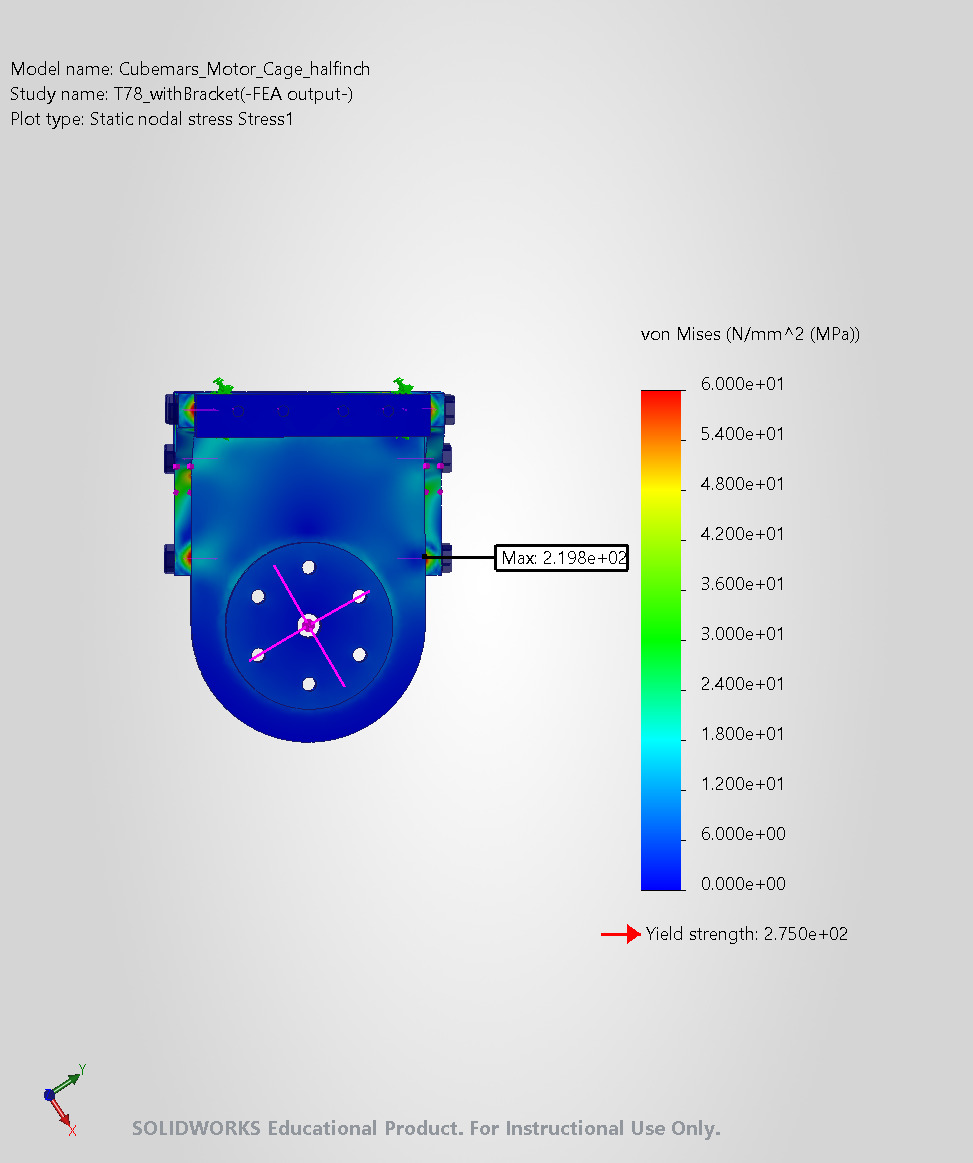
\includegraphics[width=\linewidth]{withBracket_coarse_stress_max.jpg}
  \caption{Coarse, max 219.8 MPa.}
\end{subfigure}\hfill
\begin{subfigure}[t]{0.32\linewidth}\centering
  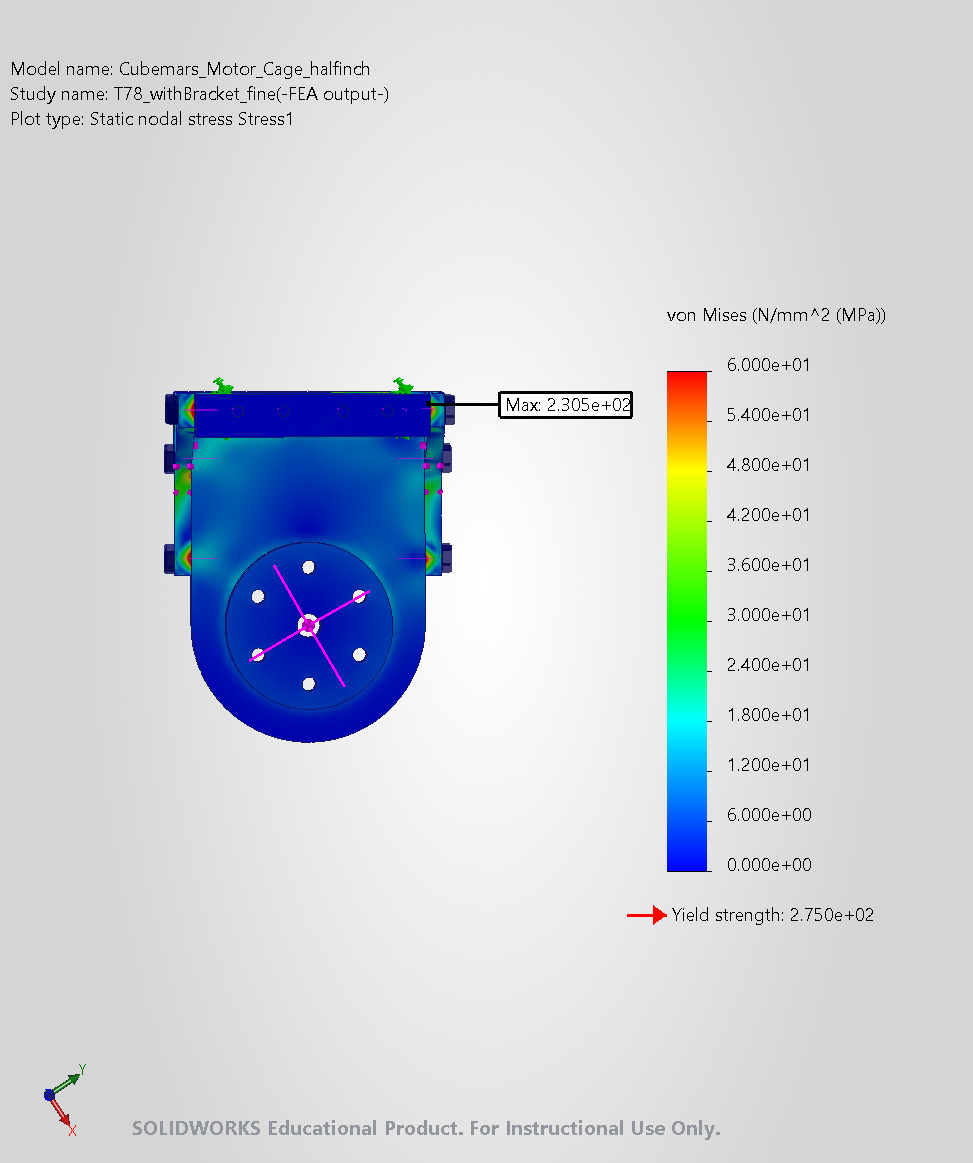
\includegraphics[width=\linewidth]{withBracket_fine_stress_max.jpg}
  \caption{Fine, max 230.5 MPa.}
\end{subfigure}\hfill
\begin{subfigure}[t]{0.32\linewidth}\centering
  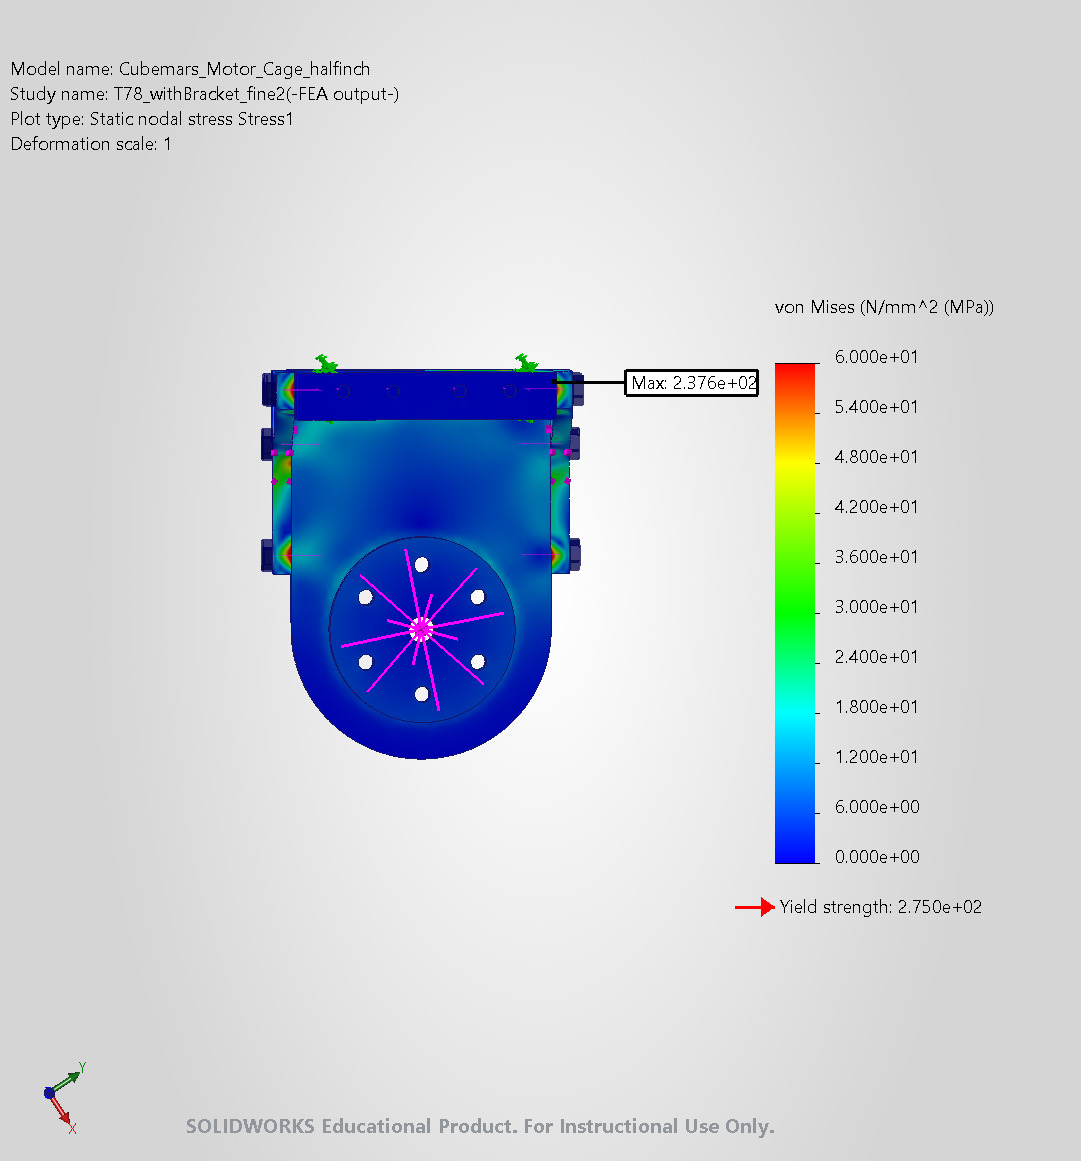
\includegraphics[width=\linewidth]{withBracket_fine2_stress_max.jpg}
  \caption{Fine2, max 237.6 MPa.}
\end{subfigure}
\caption{Location of the global stress maximum for the three meshes. It moves between
singular points and keeps rising with refinement.}
\end{figure}

\begin{figure}[H]
\centering
\begin{subfigure}[t]{0.32\linewidth}\centering
  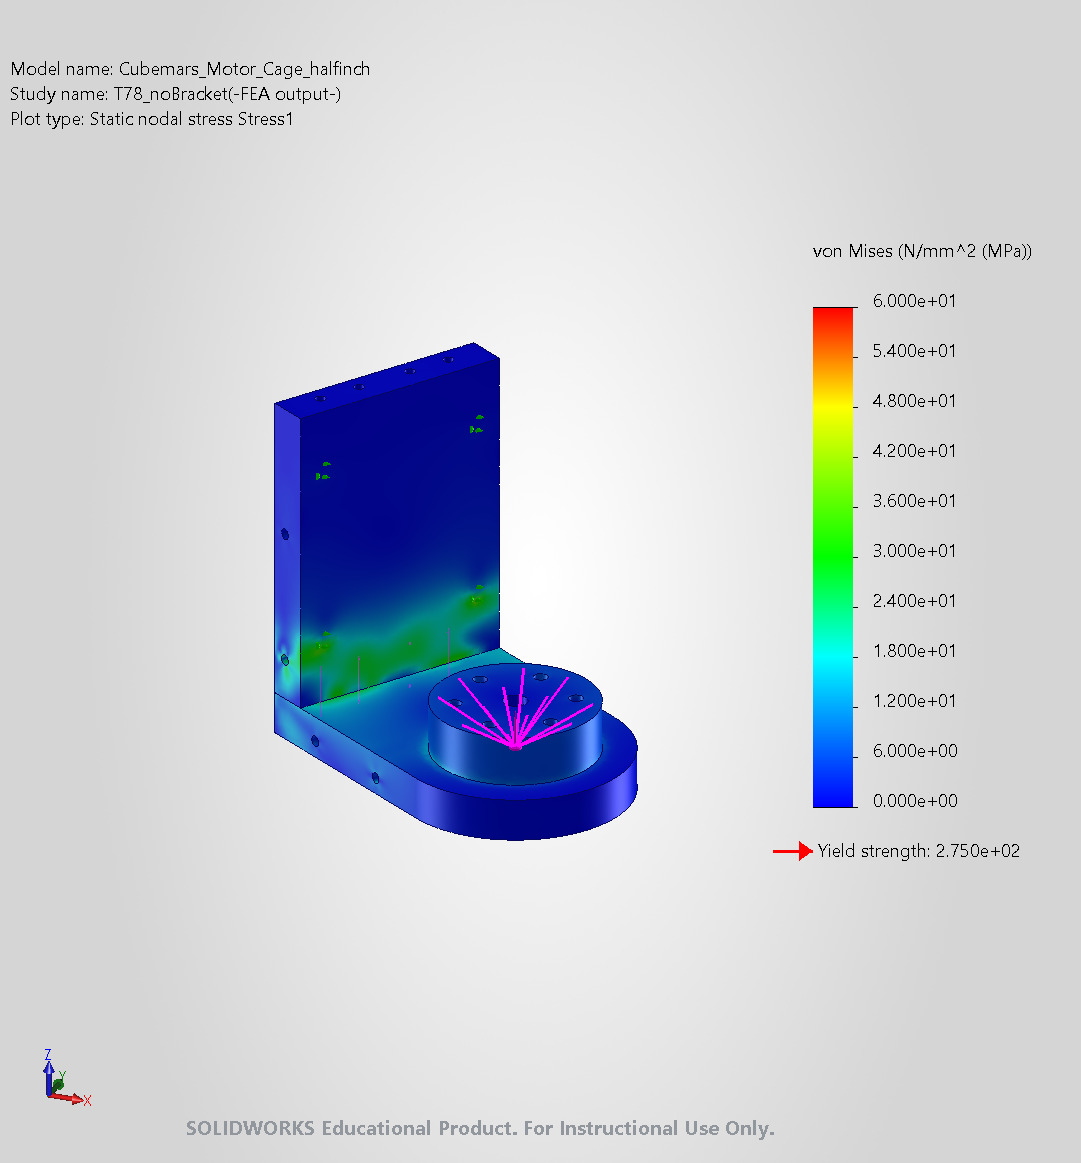
\includegraphics[width=\linewidth]{noBracket_coarse_stress_iso.jpg}
  \caption{Without brackets, von Mises, \SIrange{0}{60}{MPa}.}
\end{subfigure}\hfill
\begin{subfigure}[t]{0.32\linewidth}\centering
  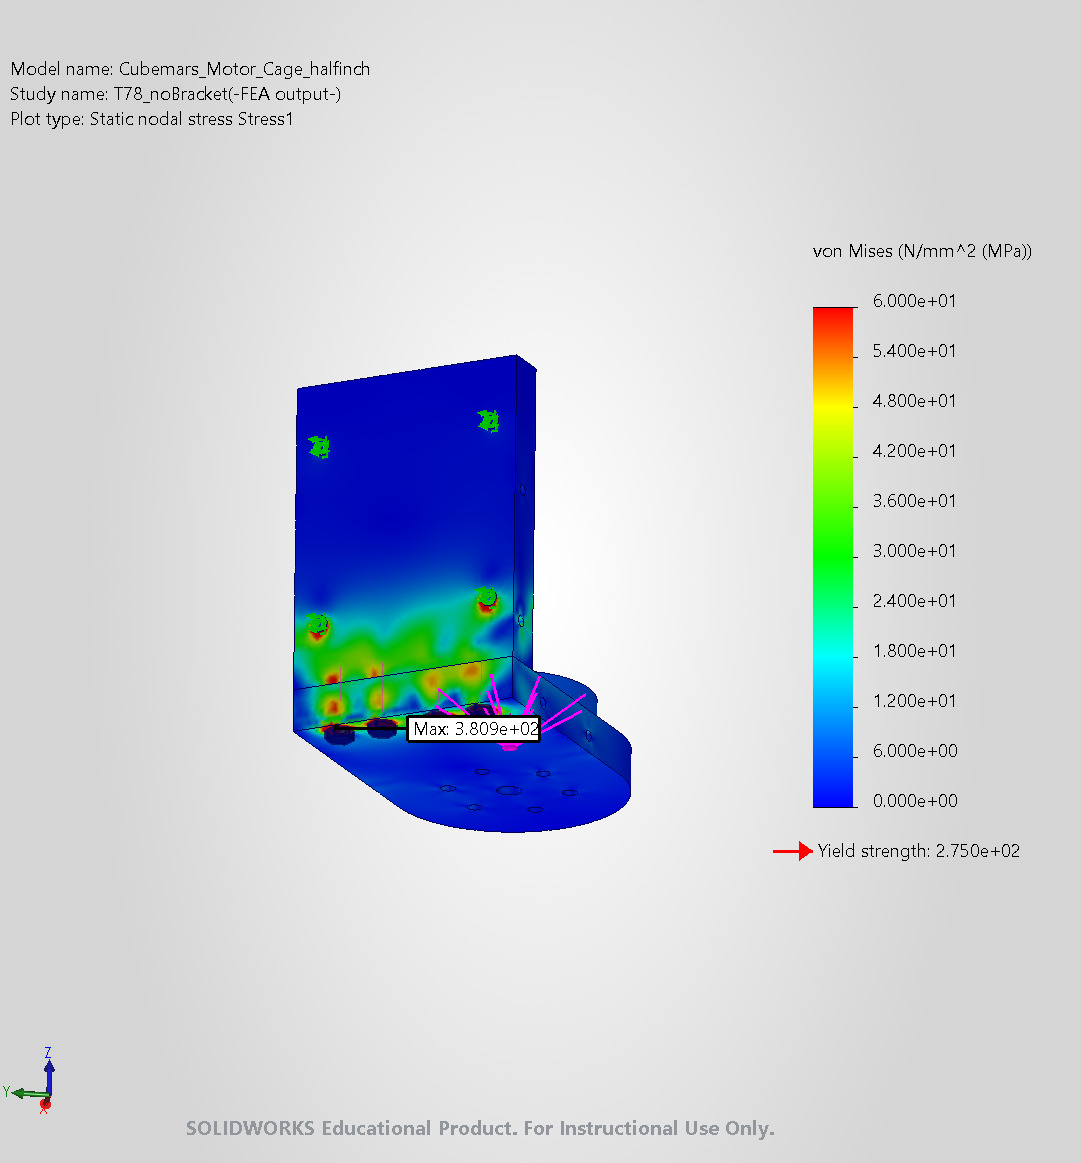
\includegraphics[width=\linewidth]{noBracket_coarse_stress_max.jpg}
  \caption{Without brackets, global max 380.9 MPa at a bolt connector.}
\end{subfigure}\hfill
\begin{subfigure}[t]{0.32\linewidth}\centering
  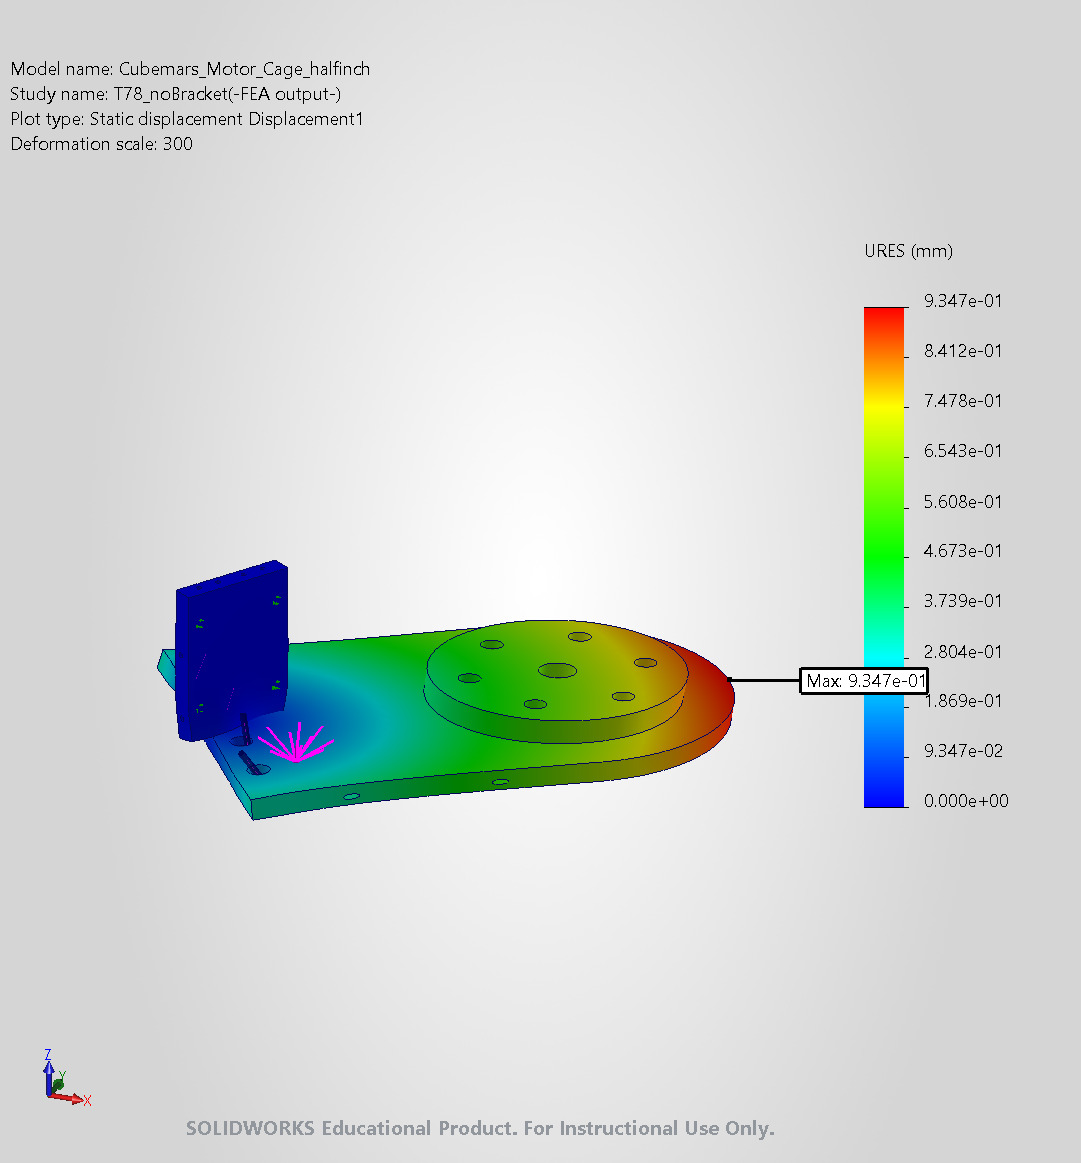
\includegraphics[width=\linewidth]{noBracket_coarse_disp_iso.jpg}
  \caption{Without brackets, displacement, $300\times$.}
\end{subfigure}
\caption{Without-bracket study, coarse mesh.}
\end{figure}

\end{document}
